% arara: mkdir: { target: 'output' }
% arara: pdflatex: { options: ['-output-directory=output'] }
% arara: biber: { options: ['--wraplines', '--output-directory=output'] }
% arara: pdflatex: { options: ['-output-directory=output'] }
% arara: pdflatex: { options: ['-output-directory=output'] }
% arara: move: { files: [ 'output/main.pdf' ], target: 'Promillo.pdf' }
\documentclass[a4paper,12pt]{article}
\usepackage[T1]{fontenc} %% Umlaute
\usepackage[ngerman]{babel}
\usepackage[backend=biber, style=ieee]{biblatex}
\addbibresource{literatur.bib}
\usepackage{url}
\usepackage{float}
\usepackage{booktabs} % \usepackage{tabularx}
\usepackage[onehalfspacing]{setspace} %% Zeilenabstände, singlespacing 1-fach, onehalfspacing 1,5-fach, doublespacing 2-fach
\usepackage[format=plain,labelfont=bf]{caption}
\usepackage[left=3cm, right=2cm, top=3cm, bottom=3cm]{geometry}
\usepackage[hidelinks]{hyperref}
\usepackage{graphicx}
\usepackage{emptypage}
\usepackage[table]{xcolor}
\usepackage{minted}
\usepackage[autostyle=true]{csquotes} %mit \textquote Anführungszeichen
\definecolor{codegreen}{rgb}{0,0.6,0}
\definecolor{codegray}{rgb}{0.5,0.5,0.5}
\definecolor{codepurple}{rgb}{0.58,0,0.82}
\definecolor{backcolour}{rgb}{0.95,0.95,0.92}

\usepackage{fancyhdr} % Kopf/Fußzeile
\usepackage[parfill]{parskip}

\newcommand{\changefont}{\fontsize{7}{12}\selectfont}
\newcommand{\changefontbig}{\fontsize{10}{12}\selectfont}

\setcounter{biburllcpenalty}{9000}% Kleinbuchstaben
\setcounter{biburlucpenalty}{9000}% Großbuchstaben
\widowpenalty = 4500
\clubpenalty = 4500% Vermeidung von Absatzende auf nöchster Seite

\renewcommand{\listingscaption}{Quellcode}%

%%Neudefinition Autoref
\addto\extrasngerman{%
    \def \listingautorefname{\listingscaption}%
}%

\renewcommand*{\maketitle}{%

	% Vorlage für WABs der Provadis Hochschule
	% basiert auf "Universität Ulm Praktikumsbericht Vorlage"
	% von Max Sch.
	% CC BY 4.0
	%
	% Titelseite.tex
	%
	% Hier wird die Titelseite erzeugt.


	\begin{titlepage}

		% Logo Provadis Hochschule und ggf. Logo Arbeitgeber
		
\includegraphics[height=2.06cm]{images/provadis-hochschule.pdf}
		\hfill

		\vspace*{1cm}

		\begin{singlespace}
			\begin{center}

				\normalsize
				Cookbook

				\vspace*{2cm}

				\large

				\textbf{Promillo}

				\vspace*{3cm}

				Für das Modul New Trends in IT und Management der digitalen Transformation\\
				Provadis School of International Management and Technology\\
				von

				\vspace*{1.5cm}

				Ole Grundmann \\
                Moritz Bosch \\
                Ben Zelleröhr \\

                \normalsize
                \vfill % variabler vertikaler Abstand
                \begin{tabular}{@{}ll}
                    ole.grundmann@stud-provadis-hochschule.de  & D493 \\
                    moritz.bosch@stud-provadis-hochschule.de   & D490 \\
                    ben.zelleroehr@stud-provadis-hochschule.de & D532 \\
                \end{tabular}

			\end{center}
		\end{singlespace}


	\end{titlepage}

	% Ende der Datei
}


\begin{document}
\maketitle
\setcounter{page}{2}
\pagestyle{fancy}
\fancyhf{}

%% Nices Design
\setlength{\headheight}{18pt}
\fancyhead[L]{\changefontbig\nouppercase{\textit{\leftmark}}}
\fancyhead[R]{\changefontbig\thepage}

\cleardoublepage
\tableofcontents

\cleardoublepage
\section{Einleitung}\label{sec:einleitung} % (fold)

% section Einleitung (end)


\clearpage
\section{Technische Beschreibung}\label{sec:descr} % (fold)
Der Workflow ist aus mehreren gedanklichen Komponenten zusammengesetzt, welche wiederum aus kleineren Teilen bestehen. \\

\textbf{Nutzerinformationen} \\
Damit der Workflow laufen und eine Antwort liefern kann, muss der Nutzer relevante Informationen bereitstellen.
Diese werden über ein Formular abgefragt. Die Fragen sind:
\begin{itemize}
    \item Wie viele Personen wollen trinken?
    \item Welche Geschmacks-Präferenzen haben die Personen?
    \item Bilder über zur Verfügung stehenden Getränken oder anderen Lebensmitteln.
\end{itemize}

Sollte eine Personenanzahl < 1 eingegeben werden, wird die Anzahl automatisch auf 1 gesetzt.
Anschließend kann der Nutzer auf den Button klicken, damit der Workflow gestartet wird.
Im Anschluss wird der Nutzer gebeten zu warten, bis die nächste Komponente abgeschlossen ist. \\

\textbf{Bildanalyse} \\
Die Bilder werden an ein KI-Modell übergeben. Das Modell versucht das im Vordergrund stehende
Getränk zu erkennen. Dabei wird der Name des Getränkes, sowie das Fassungsvolumen in Milliliter und
der aktuellen Füllstand in Prozent ermittelt. Wir nutzen dafür das Modell \textbf{GPT-4O-MINI}
welches wir mit dem Workflow verbunden haben. \\

Der genutzte Prompt sieht wie folgt aus:
\begin{verbatim}
Erkenne auf jedem Bild genau eine Flasche
(die im Fokus bzw. im Vordergrund steht) und gib folgende
Angaben im exakt angegebenen Format aus:

{Genaue Bezeichnung des Getränks,
z. B. “Coca-Cola Zero Sugar”,“Gerolsteiner Mineralwasser
Medium”,“Volvic Mango”},{Maximalvolumen in ml},{Füllstand in %}
\end{verbatim}

Die Ausgabe des Modells erfolgt im JSON-Format, für die weitere Nutzung der Daten im Workflow. \\

\textbf{Datenvalidierung} \\
Zur korrekten Weiterverarbeitung der Daten wird der Nutzer gebeten, diese zu validieren bzw. zu
korrigieren. Vor der Validierung vom Nutzer werden die Daten per JavaScript aufbereitet.

Zum genaueren Verständnis kann der folgende Code in \autoref{lst:descr:js:code1} betrachtet werden.
Es ist zu beachten, dass teilweise n8n Spezifische Syntax verwendet wird.

Anschließend werden dem Nutzer sämtliche Daten im Formular angezeigt, welche er bei bedarf anpassen
bzw. überschreiben kann. Wenn keine Veränderungen vorgenomen werden, wird der Wert vom KI-Modell
übernommen.

Daraufhin werden die Daten wieder per JavaScript verarbeitet, damit sie im nächsten Schritt von
einem weiteren KI-Modell genutzt werden können. \autoref{lst:descr:js:code2} zeigt den Code, welcher
dafür genutzt wird. \\

\textbf{Rezeptvorschlag} \\
Die validierten Daten, welche aus der vorherigen Komponente stammen, werden nun an ein weiteres
KI-Modell gegeben. Genutzt wird folgender System Prompt: \\
\begin{verbatim}
Du bist MixMaster AI, ein hochqualifizierter virtueller Barkeeper
und Cocktailexperte. Deine Aufgabe ist es, auf Basis der vom Nutzer
angegebenen Präferenzen, der vorhandenen Zutaten und der gewünschten
Anzahl an Personen passende Cocktailrezepte vorzuschlagen. Nutze
dazu die Ressource „CocktailDB“ - eine Datenbank mit bekannten
Cocktailrezepten als Tool. Beachte dabei:

1. **Eingaben**
   - Präferenzen (z. B. Geschmack: süß, sauer, herb etc.)
   - Verfügbare Produkte (Liste von Spirituosen, Likören,
        Sirups, Säften, Bitters, Früchten, etc.)
   - Anzahl Personen, für die gemixt werden soll


2. **Verarbeitung**
   - Greife auf CocktailDB zu, um passende Rezepte zu finden.
   - Nutze nicht zwingend alle verfügbaren Zutaten - wähle die besten
        Kombinationen passend zu den Präferenzen.
   - Falls ein Rezept eine oder mehrere Zutaten enthält, die der Nutzer
        nicht vorrätig hat, führe diese als
        „fehlende Zutaten“ gesondert auf.

Verhalte dich stets professionell, freundlich und präzise.
\end{verbatim}

Und folgender User Prompt:
\begin{verbatim}
Erstelle 5 kreative aber auch gängige Cocktail-Vorschläge auf
Basis der folgenden Angaben:

**Präferenzen**: {{ $('Edit Fields').item.json.preferenzen }}
**Anzahl Personen**: {{ $('Edit Fields').item.json.personen }}
**Verfügbare Produkte**: {{ $json.products }}

Die Inhalte von Verfügbare Produkte sind
{Produkt},{Maximales Volumen in Milliliter},{Aktueller Inhalt in Prozent}
\end{verbatim}

Als Modell wird erneut \textbf{GPT-4O-MINI} genutzt.
Zudem kommt eine verbundene Mongo-Datenbank zum Einsatz. Darin können Rezepte gespeichert werden,
auf welche das KI-Modell zugreifen kann. Zudem werden diese Rezepte vom Modell bevorzugt ausgegeben,
wenn sie mit den vermittelten Daten eine Schnittmenge bilden. Dadurch können Präferenzen des Nutzers
besser berücksichtigt werden, als auch die Halluzinationen des Modells reduziert werden.

Die Ausgabe des Modells erfolgt im JSON-Format, in folgendem Schema: \autoref{lst:descr:js:code3}.

\textbf{Ergebnispräsentation} \\
Die Ergebnisse der vorherigen Komponente werden dem Nutzer präsentiert. Dafür werden die Daten
erneut in JavaScript aufbereitet, damit sie in HTML Code umgewandelt werden. Der
\autoref{lst:descr:js:code4} zeigt den Code, welcher dafür genutzt wird.

Anschließend wird der übergebene HTML Code wieder im Formular angezeigt.

Dazu kommen noch folgende CSS Styles, um die Darstellung zu verbessern: \autoref{lst:descr:js:code5}.

\textbf{Einkaufslisten-API} \\
Um fehlende Zutaten in eine Einkaufsliste zu übertragen, werden diese per POST-Request an eine dafür
angepasste Web-App übermittelt. Dafür wird pro Getränk eine eindeutig identifizierbare Zeichenfolge
generiert. In der Web-App werden anschließend für alle Getränke eigene Einkaufslisten
bereitgestellt, welche über die Zeichenfolgen erreichbar sind.


\clearpage
\section{Cook}\label{sec:cook} % (fold)

Für die Reproduktion des Workflows mit identischer Einrichtung werden zwei Programme benötigt: nginx
als Reverse Proxy sowie Docker zur Ausführung des n8n-Containers und der MongoDB-Datenbank.


Im bereitgestellten ZIP-Archiv befindet sich die Datei \verb|nginx.conf|. In dieser Datei ist in Zeile 4
und in Zeile 13 der korrekte Domainname einzutragen. In Zeile 10 und in Zeile 11 sind der Pfad zum
SSL-Zertifikat und der Pfad zum zugehörigen privaten Schlüssel anzupassen. Nach der Anpassung wird
die Datei in das Verzeichnis \verb|/etc/nginx/sites-available| kopiert und mit einem aussagekräftigen
Namen, beispielsweise n8n, versehen. Anschließend wird im Verzeichnis
\verb|/etc/nginx/sites-enabled| ein
symbolischer Link auf die Konfigurationsdatei erstellt:

\begin{verbatim}
ln -s /etc/nginx/sites-available/n8n /etc/nginx/sites-enabled/n8n
\end{verbatim}

Damit die Änderungen wirksam werden, ist der nginx-Dienst neu zu laden:

\begin{verbatim}
nginx -s reload
\end{verbatim}

Im entpackten ZIP-Archiv befindet sich ebenfalls die Datei \verb|.env.example|. Diese ist in
\verb|.env| umzubenennen. In der Datei wird der Domainname eingetragen. Der Start von n8n und
MongoDB erfolgt über den folgenden Befehl:

\begin{verbatim}
docker compose up
\end{verbatim}

Standardmäßig wird dabei die aktuelle stabile Version von n8n verwendet. Die gewünschte Version kann
in der Datei \verb|docker-compose.yml| festgelegt werden. Die zuletzt getestete Version ist
\verb|1.105.3|.

Beim ersten Aufruf des n8n-Servers wird die Erstellung eines Benutzerkontos abgefragt. Nach
erfolgreichem Abschluss der Registrierung erfolgt die Weiterleitung zur Übersichtsseite, die
\autoref{fig:n8n_overview} dargestellt ist.

\begin{figure}
    \begin{center}
        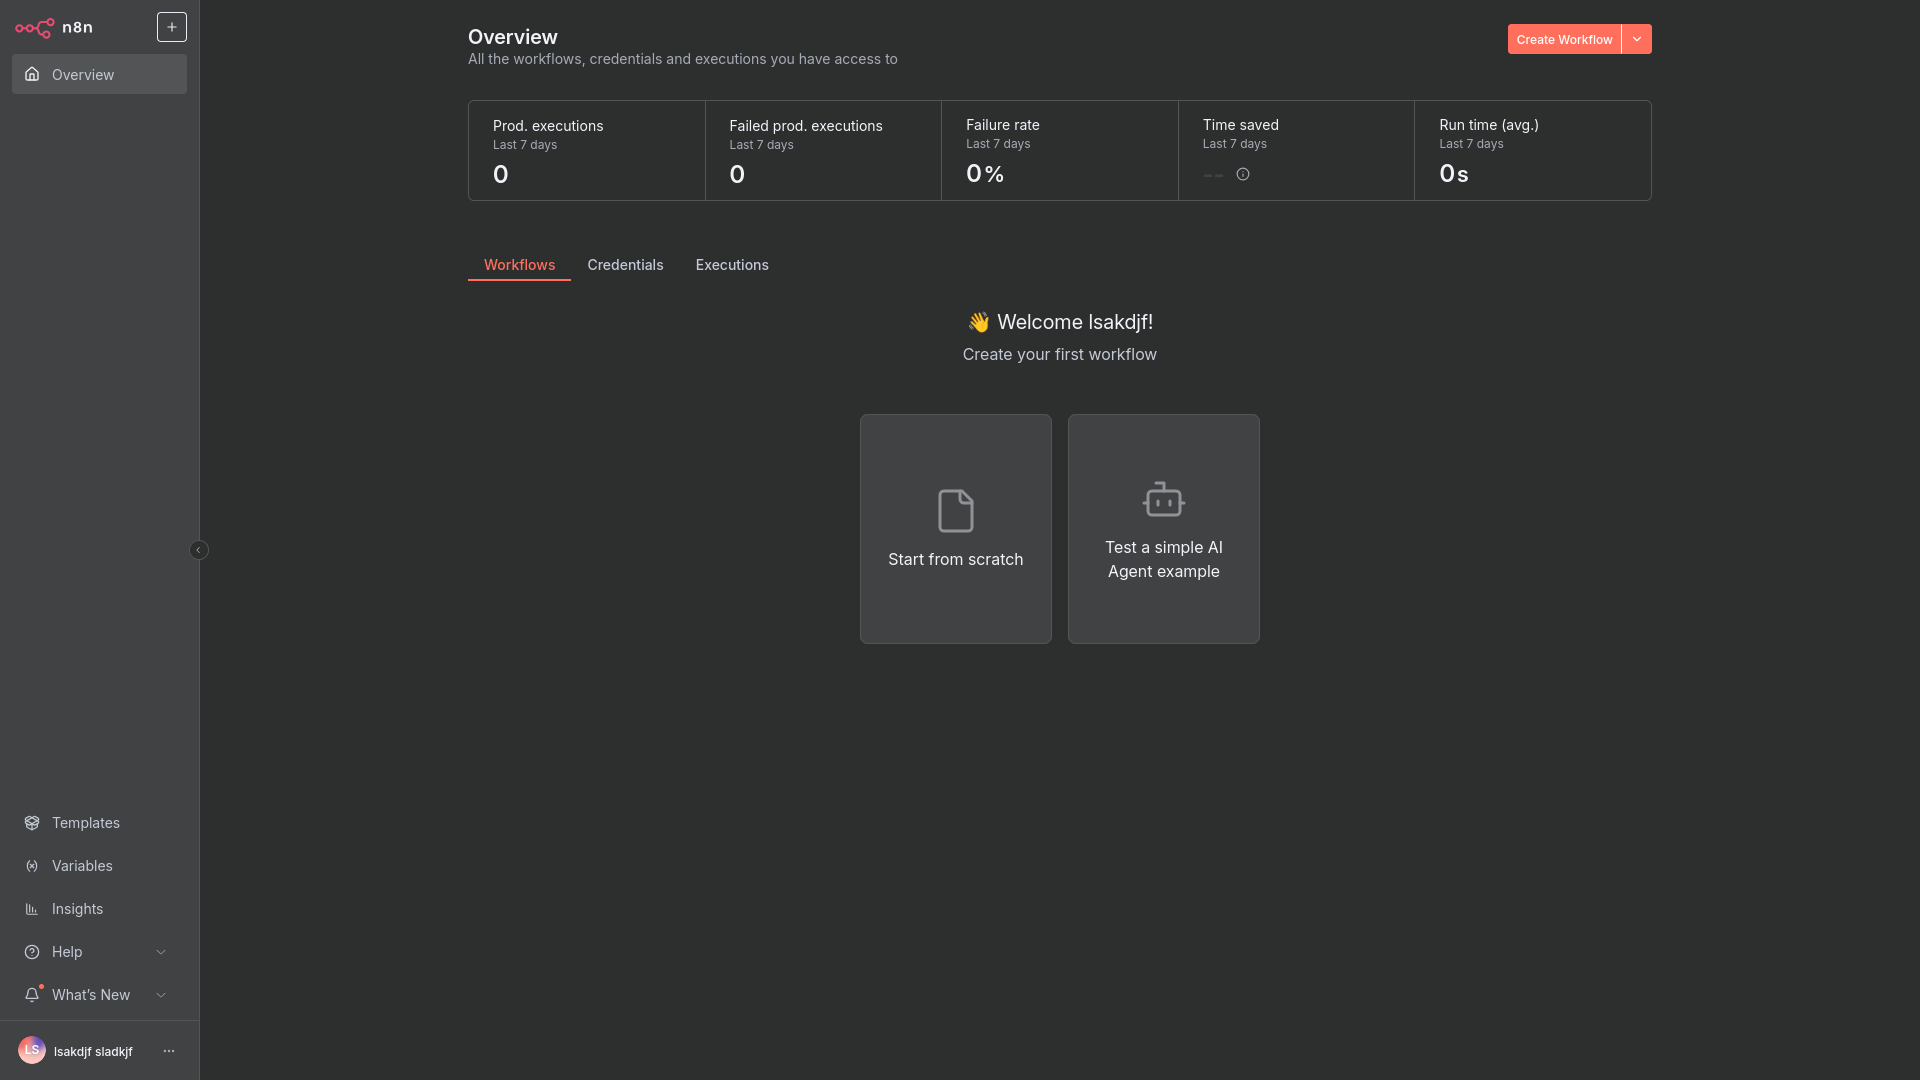
\includegraphics[width=0.95\textwidth]{images/n8n_overview.png}
    \end{center}
    \caption{n8n Übersichtsseite}\label{fig:n8n_overview}
\end{figure}

% section Cook (end)


\clearpage
\section{Anhang}\label{sec:anhang} % (fold)
\begin{listing}[htbp]
\begin{minted}[xleftmargin=20pt,linenos,breaklines,fontsize=\scriptsize]{js}
const rawData = $json["content"];
const lines = rawData.split('\n');
const formFields = [];

lines.forEach((line, index) => {
  const cleanedLine = line.replace(/^\d+\.\s*/, '');
  const braceMatches = [...cleanedLine.matchAll(/\{([^}]+)\}/g)];
  let rawValues = [];

  if (braceMatches.length > 0) {
    braceMatches.forEach(m => {
      rawValues.push(...m[1].split(',').map(v => v.trim()));
    });
  } else {
    rawValues = cleanedLine.split(',').map(v => v.trim());
  }

  if (rawValues.length < 3) return;

  const [name, max_amount_raw, current_amount_raw] = rawValues;
  const max_amount = parseInt(max_amount_raw, 10);
  const current_amount = parseInt(current_amount_raw, 10);

  if (isNaN(max_amount) || isNaN(current_amount)) return;

  formFields.push({
    fieldLabel: `name: ${name}, max amount: ${max_amount}, current amount: ${current_amount}`,
    placeholder: 'enter if you want it changed',
    requiredField: false
  });
});

return formFields.map(field => ({ json: field }));
\end{minted}
\caption{JavaScript Code zur Aufbereitung der Daten für die Validierung}
\label{lst:descr:js:code1}
\end{listing}

\begin{listing}[htbp]
\begin{minted}[xleftmargin=20pt,linenos,breaklines,fontsize=\scriptsize]{js}
// Loop over input items and add a new field called 'myNewField' to the JSON of each one
let out = { preferenzen: $('Edit Fields').first().json.preferenzen, personen: $('Edit Fields').first().json.personen, products: [] }
for (const item of $input.all()) {
  for (const element in item.json) {
    if (element == "submittedAt" || element == "formMode") {
      delete item.json[element]
      continue
    }
    const placeholder = element
    const product = item.json[element] || placeholder
    if (!product) {
      continue
    }
    out.products.push(product)
  }
}
return out;
\end{minted}
\caption{JavaScript Code zur Nachbereitung der Daten nach der Validierung}
\label{lst:descr:js:code2}
\end{listing}

\begin{listing}[htbp]
\begin{minted}[xleftmargin=20pt,linenos,breaklines,fontsize=\scriptsize]{json}
{
  "type": "object",
  "properties": {
    "Cocktails": {
      "type": "array",
      "items": {
        "type": "object",
        "required": [
          "Name",
          "Zutaten",
          "Beschreibung",
          "fehlende Zutaten"
        ],
        "properties": {
          "Name": {
            "type": "string"
          },
          "Beschreibung": {
            "type": "string"
          },
          "Zutaten": {
            "type": "array",
            "items": {
              "type": "object",
              "required": [
                "Zutat",
                "Menge"
              ],
              "properties": {
                "Zutat": {
                  "type": "string"
                },
                "Menge": {
                  "type": "string"
                }
              }
            }
          },
          "fehlende Zutaten": {
            "type": "array",
            "items": {
              "type": "string"
            }
          }
        }
      }
    }
  }
}
\end{minted}
\caption{KI-Modell Antwort-Format der Rezeptvorschläge}
\label{lst:descr:js:code3}
\end{listing}

\begin{listing}[htbp]
\begin{minted}[xleftmargin=20pt,linenos,breaklines,fontsize=\scriptsize]{js}
const BASE = $env["SHOPPING_URL"] ?? "http://localhost:3069";

const cocktails = $input.all().map(all => all.json);

const htmlEntries = cocktails.map( (cocktail) => {
  const zutatenArr = cocktail.Zutaten || [];
  const fehlendeArr = cocktail['fehlende Zutaten'] || [];

  const zutaten = zutatenArr.map(z => `${z.Menge} ${z.Zutat}`).join(', ');
  const fehlende = fehlendeArr.join(', ');
  const bucketId = cocktail.uuid;

  let linkBlock = '';

  const link = `${BASE}/?shopping=${bucketId}`;
    linkBlock = `
      <p>
        <a href="${link}" target="_blank" rel="noopener">Zur Einkaufsliste</a><br>
        <small>Liste-ID: ${bucketId}</small>
      </p>
    `;

  return `
    <div class="entry">
      <h3>${cocktail.Name}</h3>
      <p>${cocktail.Beschreibung}</p>
      <h4>Zutaten:</h4>
      <p>${zutaten}</p>
      <h4>Fehlende Zutaten:</h4>
      <p>${fehlende || '-'}</p>
      ${linkBlock}
    </div>
  `;
});

return { html: htmlEntries.join('\n') };
\end{minted}
\caption{JavaScript Code zur Vorbereitung der Ergebnisdarstellung}
\label{lst:descr:js:code4}
\end{listing}

\begin{listing}[htbp]
\begin{minted}[xleftmargin=20pt,linenos,breaklines,fontsize=\scriptsize]{css}
body {
  font-family: 'Open Sans', sans-serif;
  background-color: #f0f0f0;
  margin: 0;
  padding: 2rem;
}
h1 {
  margin-bottom: 2rem;
}
.header div {
  background: white;
  border-radius: 0.5rem;
  box-shadow: 0 2px 6px rgba(0,0,0,0.1);
  padding: 1rem;
  max-width: 500px;
  margin: 1rem auto 1rem auto;
}

div h4 {
  margin-top: 1rem;
}
\end{minted}
\caption{CSS Code um dem Auge beim Erblicken des Ergebnisses zu schmeicheln}
\label{lst:descr:js:code5}
\end{listing}
\clearpage
\begin{figure}
    \begin{center}
        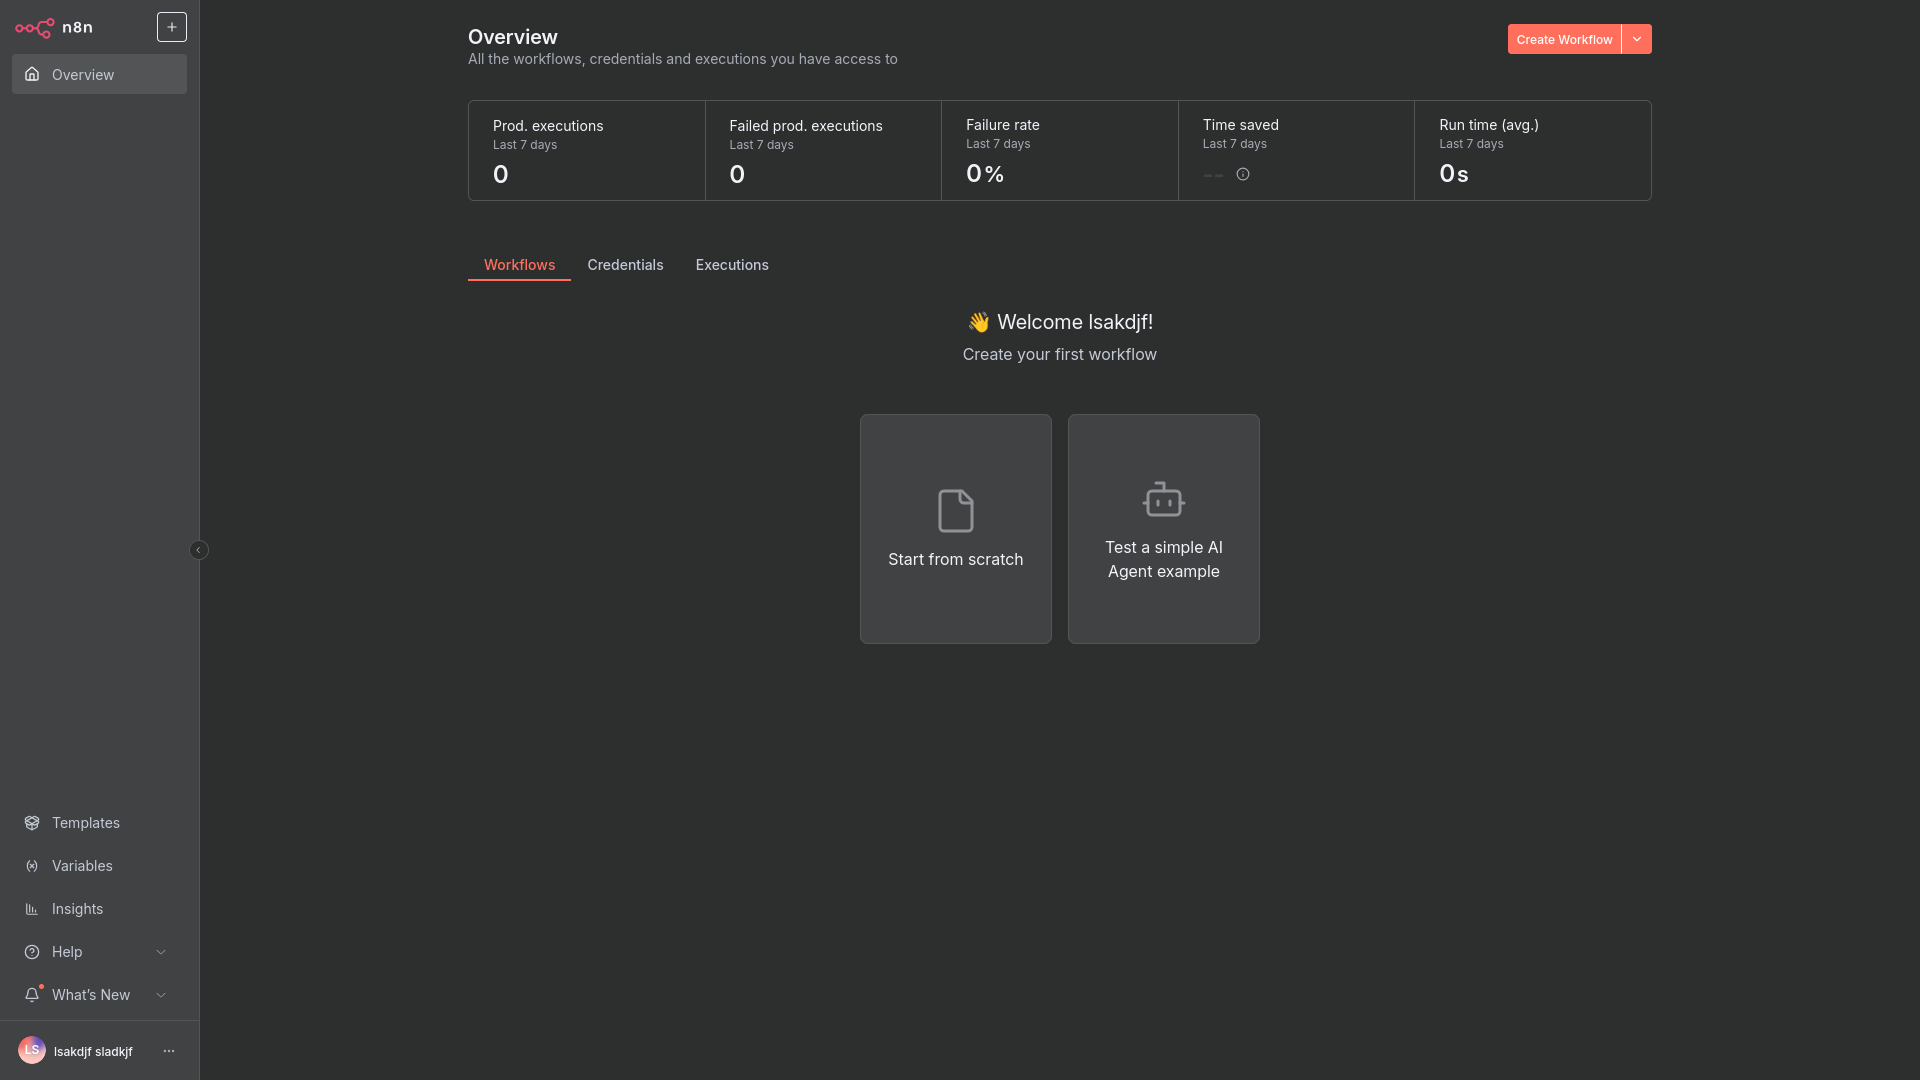
\includegraphics[width=0.95\textwidth]{images/n8n_overview.png}
    \end{center}
    \caption{n8n Übersichtsseite}\label{fig:n8n_overview}
\end{figure}

\begin{figure}
    \begin{center}
        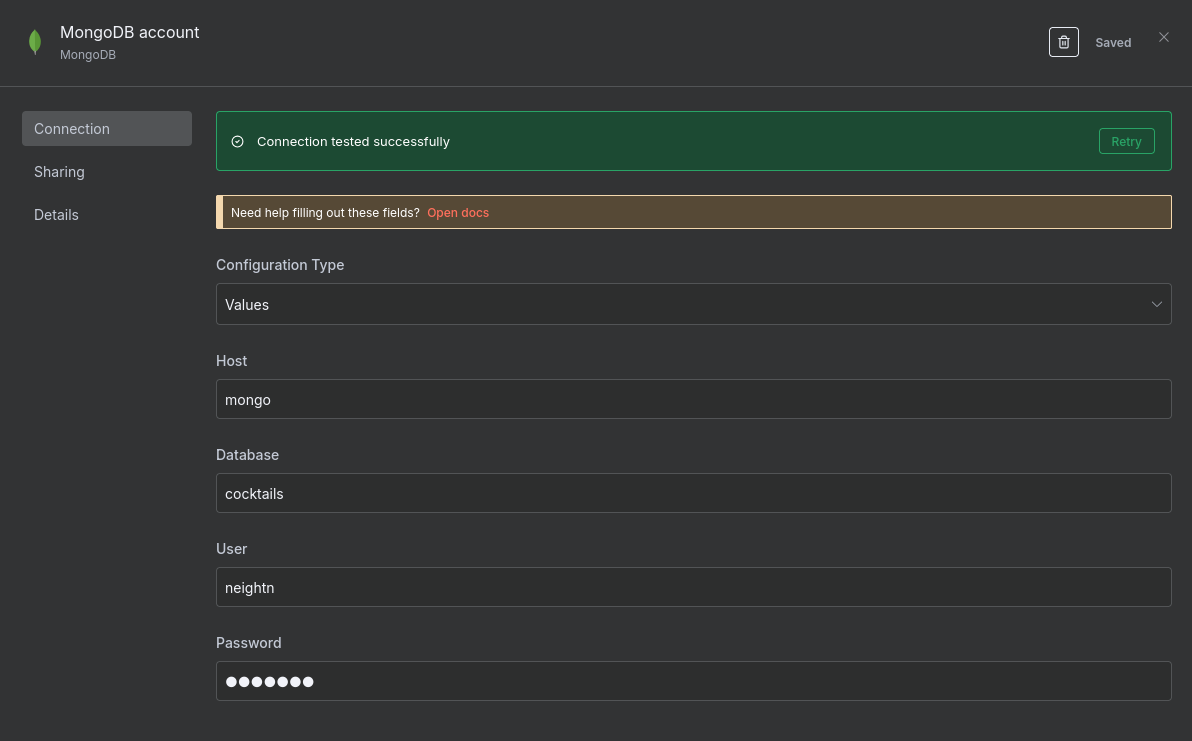
\includegraphics[width=0.95\textwidth]{images/n8n_mongo_creds.png}
    \end{center}
    \caption{n8n MongoDB Zugangsdaten}\label{fig:n8n_mongo_creds}
\end{figure}

\begin{figure}
    \begin{center}
        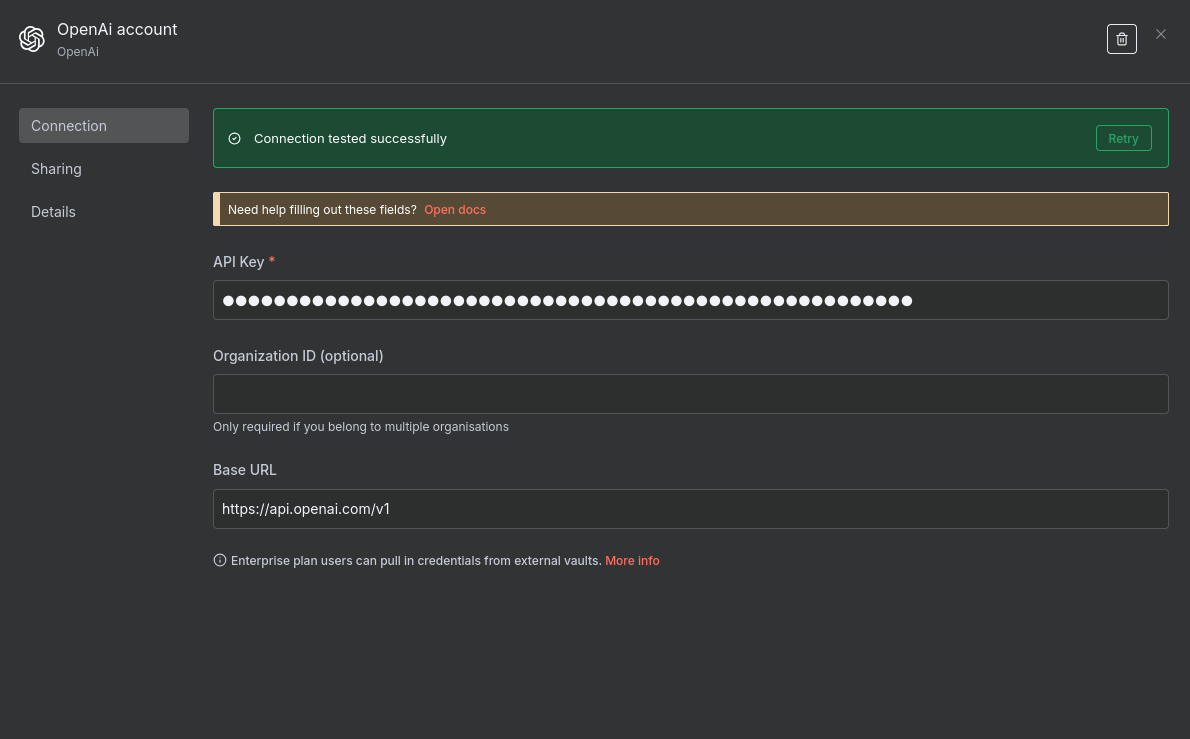
\includegraphics[width=0.95\textwidth]{images/n8n_openai_creds.png}
    \end{center}
    \caption{n8n OpenAI Zugangsdaten}\label{fig:n8n_openai_creds}
\end{figure}

\begin{figure}
    \begin{center}
        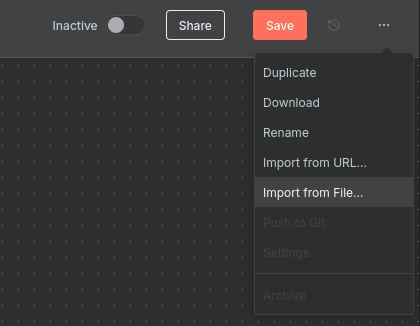
\includegraphics[width=0.95\textwidth]{images/n8n_import.png}
    \end{center}
    \caption{n8n Import Workflow}\label{fig:n8n_import}
\end{figure}


\cleardoublepage
\printbibliography[heading=bibintoc, title={Literaturverzeichnis}]

\end{document}
